% https://nathantypanski.com/blog/2014-10-29-tikz-timing.html
% https://github.com/yne/vcd (the C one for the terminal)
% https://github.com/martonbognar/vcdvis (the Python one for Tikz)
% https://github.com/ernstblecha/vcd2tikztiming (another Python one)
% https://github.com/wifasoi/WaveDromTikZ (another Python one but for WaveDrom files)
% https://en.wikipedia.org/wiki/Value_change_dump
% https://ctan.org/tex-archive/graphics/pgf/contrib/tikz-timing?lang=en
\documentclass{article}

\title{Implementing various adders in Verilog}
\author{Diego Bellani - 1838645}
\date{2023}

\usepackage[hidelinks]{hyperref}
\usepackage{tikz}

\begin{document}

\maketitle

\begin{abstract}
We implemented some classic digital adders, and some others based on non
standard number systems, in Verilog using delayed gates to have a somewhat
realistic simulation.

The aim of this project was mainly pedagogical, to see how effective the various
strategies to implement addition are and also to see how reasonable they are to
implement at this level of detail.

All the adder have also been verified to be correct by and exhaustive search
over all possible 8-bit number.
\end{abstract}

\section{Introduction}

Addition is a fundamental mathematical operation and it is a cornerstone of all
numerical algorithms. Having a fast implementation of this operation is crucial
if we want to implement this kind of algorithms in a performant way. The main
obstacle to a fast implementation of addition in hardware is the wait for carry
propagation.

In this project we implemented (and simulated) various digital addition
strategies in the Verilog hardware description language, at the logic gate
level, making sure that all gates had a uniform delay. While this is not a
realistic assumption it is still a good pedagogical tool to show how the
propagation of the signals happens in a digital circuit.

We implemented the following classical adders: ripple-carry, carry-select,
carry-lookahead and serial adder. We also implemented adders based on a residue
number system and a redundant number system with signed digits, we are going to
call this two adders the ``non standard'' ones.

Even under our simplifying assumptions we had some surprising results. Like the
fact that some supposedly faster circuits are not always the best performing,
which is not obvious at all when studying them on paper.

\section{Implementation}

All classical adders were implemented as modules parametric in the number of
bits that they add. The only exception was the carry-lookahead adder which
(given the meta-programming capabilities of Verilog) we could not implement in
this parametric fashion, so we settled for a fixed width implementation. To
somewhat remediate to this we implemented another adder based on the recursive
relation (without unrolling) of the carry-lookahead adder i.e.

\begin{displaymath}
C_i = G_{i-1} + P_{i-1} \cdot C_{i-1}\mathrm.
\end{displaymath}

We called this adder the carry-lookahead slow.

One of the non standard adders is instead parametric in the numbers of
``digits'' it adds and the other in parametric in the exponent used to generate
the set of moduli. This did not allow us to perform a totally fair comparison
between the two category of adders since they could add different ranges of
numbers(in particular this category of adders ended up being able to add a
slightly bigger range than the standard ones).

All the adders are implemented at the logic gate level (or register-transfer
level). The only exception is the serial adder because Verilog does not allow
for edge triggering at the gate level and forces you to use behavioral
construct instead. This is not as bad as it sounds since the serial adder always
take fixed number of clock cycles add the numbers therefore if was always going
to be the slowest.

To make verification feasible we decided to limit ourselves to adder who could
at least add 8-bit numbers (modulo 256).

Before implementing the residue number system adder~\cite{rns} we gave a quick
look around at the literature to see which base was the ``best'' to use. Given
their popularity we initially thought to use $\{2^n+1, 2^n, 2^n-1\}$, because
implementing a modulo $2^n$ adder is trivial and an adder modulo $2^n-1$ only
requires loop around carry. After looking at~\cite{modular1, modular2,
modular3} we convinced ourselves that implementing a performant $2^n+1$ modular
adder was not an easy task. Therefore we looked around for another basis to use
and found~\cite{residue}, in which the basis $\{2^n, 2^n-1, 2^{n-1}-1\}$ is
described and it was perfect for our needs.

The redundant number system we decided to use is the quaternary signed digit.
This is because of the ease of representation of the range of its digits with
3-bit 2's complement numbers.

To implement the quaternary signed digit adder we started by
reading~\cite{qsd_blog} that cited~\cite{qsd1} and~\cite{qsd2}. From~\cite{qsd1}
we implemented the algorithm to do the number conversions, while
from~\cite{qsd2} we took the minimized boolean expression needed for the two
step addition process needed by redundant number systems.

A final remark about the non standard adder is that they require their inputs to
be converted from the classic binary format to their particular representation,
and the opposite process must be done to their outputs. This is usually their
bigger problem that stops them from being used in traditional digital computers.

In order to level the playing field for non standard adder we decided to
implement this conversions to-and-from without delays.

\section{Results}

We now present some example waveforms generated by the simulator to perform some
additions on the numbers which are labeled as $A$ and $B$. In the figures we
label the various adders with the abbreviated names found in
table~\ref{tab:abbreviations}. We are going to use the abbreviated names for the
adders in the rest of this report.

\begin{table}
\centering
\begin{tabular}{|l|l|}
\hline \textbf{Adder} & \textbf{Abbreviation} \\
\hline ripple-carry & rca \\
\hline carry-select & csa \\
\hline carry-lookahead & cla \\
\hline carry-lookahead slow & cla\_s \\
\hline residue number system & rnsa \\
\hline quaternary signed digit & qsda \\
\hline serial & sa \\
\hline
\end{tabular}
\caption{Abbreviations used in the figures for the adders.}
\label{tab:abbreviations}
\end{table}

Let us start by looking at figure~\ref{fig:wf_8p3}. The first three adders show
pretty much expected behavior, with the cla being faster than the other two.
We can already see some surprising behaviors with both rnsa and qsda having the
same speed as rca, which one would naively expect the former two be faster.

Now let us take a look at figure~\ref{fig:wf_31p31} were we find pretty much the
opposite situation. In this case the cla is the second slowest, and rnsa is
among the fastest ones.

Finally we will look at figure~\ref{fig:wf_15p9} where qsda is now one of the
two fastest adder together with cla.

This clearly shows that it is hard to see how an adder is going to perform a
priori (except for sa which, of course, is the slowest in all the cases).

\section{Conclusions}

Our examples are a bit cherry picked and not representative of the general
speed of the various adders, but some of the adders, in our limited experience,
seemed to be better in most scenarios. In particular the qsda and rnsa often
seemed to be slower than the classic cla.

This fact goes against the common knowledge, that says that this carry free
adders are supposed to be faster that the classical ones. But, as we have said
before, this is just our limited experience.

To be sure that qsda and rnsa are actually slower than cla in adding 8-bit
numbers a deeper analysis could be done by analyzing the VCD file of the
simulation directly do get the average and maximum propagation delay for all the
adders.

If this would actually be the case it would be interesting to see how big the
numbers to add have to be before we start to see the advantage of this carry
free adders.

% TODO: spiegare perché ho usato quaternary come redundant number system.
\newpage

\bibliographystyle{plain}
\bibliography{report}

\newpage\pdfpageattr{/Rotate 90}

\begin{figure}
\centering
\begin{tikzpicture}[scale=0.5, rotate=90, transform shape]
\input{8p3wf}
\end{tikzpicture}
\caption{Waveforms of all the adders for $8+3$.}
\label{fig:wf_8p3}
\end{figure}

\begin{figure}
\centering
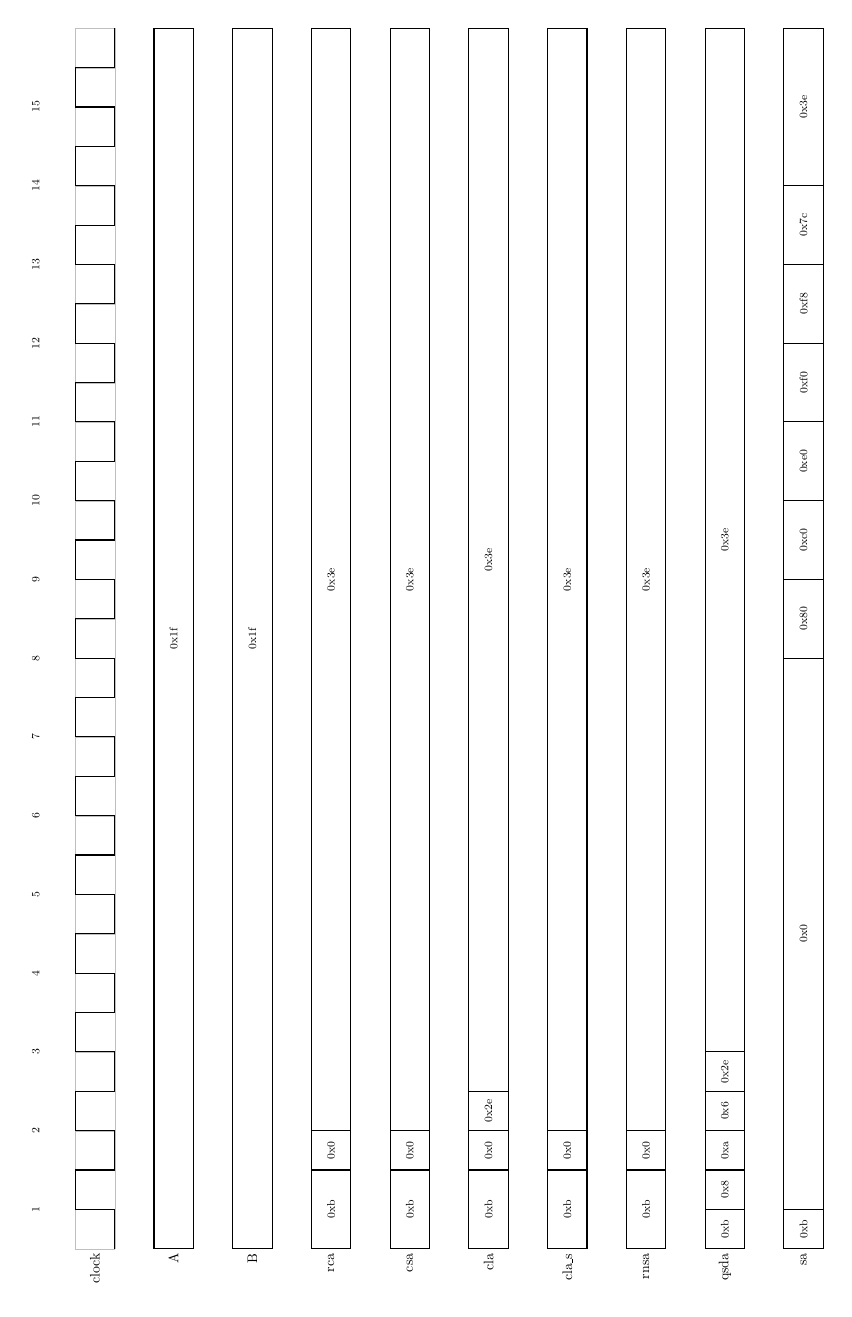
\begin{tikzpicture}[scale=0.5, rotate=90, transform shape]
\node at (1, 2) {\footnotesize 1};
\node at (3, 2) {\footnotesize 2};
\node at (5, 2) {\footnotesize 3};
\node at (7, 2) {\footnotesize 4};
\node at (9, 2) {\footnotesize 5};
\node at (11, 2) {\footnotesize 6};
\node at (13, 2) {\footnotesize 7};
\node at (15, 2) {\footnotesize 8};
\node at (17, 2) {\footnotesize 9};
\node at (19, 2) {\footnotesize 10};
\node at (21, 2) {\footnotesize 11};
\node at (23, 2) {\footnotesize 12};
\node at (25, 2) {\footnotesize 13};
\node at (27, 2) {\footnotesize 14};
\node at (29, 2) {\footnotesize 15};
\draw [help lines,lightgray,line width=0.01mm] (0,0) grid (31,1);
\draw [black] (0,0) -- (1,0);
\draw [black] (1,1) -- (2,1);
\draw [black] (1,0) -- (1,1);
\draw [black] (2,0) -- (3,0);
\draw [black] (2,0) -- (2,1);
\draw [black] (3,1) -- (4,1);
\draw [black] (3,0) -- (3,1);
\draw [black] (4,0) -- (5,0);
\draw [black] (4,0) -- (4,1);
\draw [black] (5,1) -- (6,1);
\draw [black] (5,0) -- (5,1);
\draw [black] (6,0) -- (7,0);
\draw [black] (6,0) -- (6,1);
\draw [black] (7,1) -- (8,1);
\draw [black] (7,0) -- (7,1);
\draw [black] (8,0) -- (9,0);
\draw [black] (8,0) -- (8,1);
\draw [black] (9,1) -- (10,1);
\draw [black] (9,0) -- (9,1);
\draw [black] (10,0) -- (11,0);
\draw [black] (10,0) -- (10,1);
\draw [black] (11,1) -- (12,1);
\draw [black] (11,0) -- (11,1);
\draw [black] (12,0) -- (13,0);
\draw [black] (12,0) -- (12,1);
\draw [black] (13,1) -- (14,1);
\draw [black] (13,0) -- (13,1);
\draw [black] (14,0) -- (15,0);
\draw [black] (14,0) -- (14,1);
\draw [black] (15,1) -- (16,1);
\draw [black] (15,0) -- (15,1);
\draw [black] (16,0) -- (17,0);
\draw [black] (16,0) -- (16,1);
\draw [black] (17,1) -- (18,1);
\draw [black] (17,0) -- (17,1);
\draw [black] (18,0) -- (19,0);
\draw [black] (18,0) -- (18,1);
\draw [black] (19,1) -- (20,1);
\draw [black] (19,0) -- (19,1);
\draw [black] (20,0) -- (21,0);
\draw [black] (20,0) -- (20,1);
\draw [black] (21,1) -- (22,1);
\draw [black] (21,0) -- (21,1);
\draw [black] (22,0) -- (23,0);
\draw [black] (22,0) -- (22,1);
\draw [black] (23,1) -- (24,1);
\draw [black] (23,0) -- (23,1);
\draw [black] (24,0) -- (25,0);
\draw [black] (24,0) -- (24,1);
\draw [black] (25,1) -- (26,1);
\draw [black] (25,0) -- (25,1);
\draw [black] (26,0) -- (27,0);
\draw [black] (26,0) -- (26,1);
\draw [black] (27,1) -- (28,1);
\draw [black] (27,0) -- (27,1);
\draw [black] (28,0) -- (29,0);
\draw [black] (28,0) -- (28,1);
\draw [black] (29,1) -- (30,1);
\draw [black] (29,0) -- (29,1);
\draw [black] (30,0) -- (31,0);
\draw [black] (30,0) -- (30,1);
\node [left] at (0,0.5) {clock};
\draw [black] (0,-2) rectangle (31,-1);
\node at (15.5,-1.5) {\footnotesize{0x1f}};
\node [left] at (0,-1.5) {A};
\draw [black] (0,-4) rectangle (31,-3);
\node at (15.5,-3.5) {\footnotesize{0x1f}};
\node [left] at (0,-3.5) {B};
\draw [black] (0,-6) rectangle (2,-5);
\node at (1.0,-5.5) {\footnotesize{0xb}};
\draw [black] (2,-6) rectangle (3,-5);
\node at (2.5,-5.5) {\footnotesize{0x0}};
\draw [black] (3,-6) rectangle (31,-5);
\node at (17.0,-5.5) {\footnotesize{0x3e}};
\node [left] at (0,-5.5) {rca};
\draw [black] (0,-8) rectangle (2,-7);
\node at (1.0,-7.5) {\footnotesize{0xb}};
\draw [black] (2,-8) rectangle (3,-7);
\node at (2.5,-7.5) {\footnotesize{0x0}};
\draw [black] (3,-8) rectangle (31,-7);
\node at (17.0,-7.5) {\footnotesize{0x3e}};
\node [left] at (0,-7.5) {csa};
\draw [black] (0,-10) rectangle (2,-9);
\node at (1.0,-9.5) {\footnotesize{0xb}};
\draw [black] (2,-10) rectangle (3,-9);
\node at (2.5,-9.5) {\footnotesize{0x0}};
\draw [black] (3,-10) rectangle (4,-9);
\node at (3.5,-9.5) {\footnotesize{0x2e}};
\draw [black] (4,-10) rectangle (31,-9);
\node at (17.5,-9.5) {\footnotesize{0x3e}};
\node [left] at (0,-9.5) {cla};
\draw [black] (0,-12) rectangle (2,-11);
\node at (1.0,-11.5) {\footnotesize{0xb}};
\draw [black] (2,-12) rectangle (3,-11);
\node at (2.5,-11.5) {\footnotesize{0x0}};
\draw [black] (3,-12) rectangle (31,-11);
\node at (17.0,-11.5) {\footnotesize{0x3e}};
\node [left] at (0,-11.5) {cla\_s};
\draw [black] (0,-14) rectangle (2,-13);
\node at (1.0,-13.5) {\footnotesize{0xb}};
\draw [black] (2,-14) rectangle (3,-13);
\node at (2.5,-13.5) {\footnotesize{0x0}};
\draw [black] (3,-14) rectangle (31,-13);
\node at (17.0,-13.5) {\footnotesize{0x3e}};
\node [left] at (0,-13.5) {rnsa};
\draw [black] (0,-16) rectangle (1,-15);
\node at (0.5,-15.5) {\footnotesize{0xb}};
\draw [black] (1,-16) rectangle (2,-15);
\node at (1.5,-15.5) {\footnotesize{0x8}};
\draw [black] (2,-16) rectangle (3,-15);
\node at (2.5,-15.5) {\footnotesize{0xa}};
\draw [black] (3,-16) rectangle (4,-15);
\node at (3.5,-15.5) {\footnotesize{0x6}};
\draw [black] (4,-16) rectangle (5,-15);
\node at (4.5,-15.5) {\footnotesize{0x2e}};
\draw [black] (5,-16) rectangle (31,-15);
\node at (18.0,-15.5) {\footnotesize{0x3e}};
\node [left] at (0,-15.5) {qsda};
\draw [black] (0,-18) rectangle (1,-17);
\node at (0.5,-17.5) {\footnotesize{0xb}};
\draw [black] (1,-18) rectangle (15,-17);
\node at (8.0,-17.5) {\footnotesize{0x0}};
\draw [black] (15,-18) rectangle (17,-17);
\node at (16.0,-17.5) {\footnotesize{0x80}};
\draw [black] (17,-18) rectangle (19,-17);
\node at (18.0,-17.5) {\footnotesize{0xc0}};
\draw [black] (19,-18) rectangle (21,-17);
\node at (20.0,-17.5) {\footnotesize{0xe0}};
\draw [black] (21,-18) rectangle (23,-17);
\node at (22.0,-17.5) {\footnotesize{0xf0}};
\draw [black] (23,-18) rectangle (25,-17);
\node at (24.0,-17.5) {\footnotesize{0xf8}};
\draw [black] (25,-18) rectangle (27,-17);
\node at (26.0,-17.5) {\footnotesize{0x7c}};
\draw [black] (27,-18) rectangle (31,-17);
\node at (29.0,-17.5) {\footnotesize{0x3e}};
\node [left] at (0,-17.5) {sa};


\end{tikzpicture}
\caption{Waveforms of all the adders for $31+31$.}
\label{fig:wf_31p31}
\end{figure}

\begin{figure}
\centering
\begin{tikzpicture}[scale=0.5, rotate=90, transform shape]
\input{15p9wf}
\end{tikzpicture}
\caption{Waveforms of all the adders for $15+9$.}
\label{fig:wf_15p9}
\end{figure}

\end{document}
